\documentclass[12pt]{article}

% Language setting
% Replace `english' with e.g. `spanish' to change the document language
\usepackage[english]{babel}

% Set page size and margins
% Replace `letterpaper' with`a4paper' for UK/EU standard size
\usepackage[letterpaper,top=2cm,bottom=2cm,left=3cm,right=3cm,marginparwidth=1.75cm]{geometry}


%AMS-TeX packages
\usepackage{amssymb,amsmath,amsthm} 
\usepackage{geometry, graphicx}
\usepackage{tabulary}
\usepackage{physics}
\usepackage{enumitem}


% setup the margins
\geometry{margin=1.0in, headheight=15pt}

\usepackage[colorlinks=true, allcolors=blue]{hyperref}
%% Common Declarations %%


\title{PHSX 425, HW 09}
\author{William Jardee}

\begin{document}
\maketitle

\section*{Question 1}
\emph{consider the 3D scalar wave equation}
\[\laplacian{f} = \frac{1}{v^2}\pdv[2]{f}{t}\]
\emph{Find the general solution $f(x,y,x,t)$, in terms of complex exponentials, by separation of variables.}\bigskip

Let's start by saying that $f$ is seperable, that is
\[f(x,y,x,t)=f_x(x)f_y(y)f_z(z)f_t(t)\]
\bigskip

\[\Big[\pdv[2]{x} + \pdv[2]{y} + \pdv[2]{z}\Big]f_x(x)f_y(y)f_z(z)f_t(t) = \frac{1}{v^2}\pdv[2]{t}f_x(x)f_y(y)f_z(z)f_t(t)\]
\[f_t\Big[f_y f_z\pdv[2]{f_x}{x} + f_x f_z\pdv[2]{f_y}{y} + f_x f_y\pdv[2]{f_z}{z}\Big] = f_xf_yf_z\pdv[2]{f_t}{t}\]
\[\frac{1}{f_x}\pdv[2]{f_x}{x} + \frac{1}{f_y}\pdv[2]{f_y}{y} + \frac{1}{f_z}\pdv[2]{f_z}{z} = \frac{1}{v^2}\frac{1}{f_t}\pdv[2]{f_t}{t}\]

Since the left and right side sides have to be equal for all spacial and temporal setups, let us say that they both have to be $k^2$, where $k \in \mathbb{C}$. Let's tackle the right hand side first.
\[\frac{1}{v^2}\frac{1}{f_t}\pdv[2]{f_t}{t} = k^2\]
\[\pdv[2]{f_t}{t} = k^2 v^2 f_t\]
\[\Rightarrow f_t(t) = A_t e^{kvt} + B_t e^{-kvt}\]

Now to catch the right side.
\[\frac{1}{f_x}\pdv[2]{f_x}{x} + \frac{1}{f_y}\pdv[2]{f_y}{y} + \frac{1}{f_z}\pdv[2]{f_z}{z} = k^2\]
Since this has to be true for all $x$, $y$, and $z$, then let's just say that 
\[k^2 = k_x^2 + k_y^2 + k_z^2\]
The derivation then becomes identical for all three:
\[\frac{1}{f_x}\pdv[2]{f_x}{x} = k_x^2\]
\[\pdv[2]{f_x}{x} = k_x^2 f_x\]
\[\Rightarrow f_x(x) = A_x e^{k_x x} + B_x e^{-k_x x}\]
\bigskip

Putting this all together to get one real big equation:
\begin{align*}
f(x,y,z,t) = \Big(A_x e^{k_x x} + B_x e^{-k_x x}\Big)\Big(A_y e^{k_y y} + B_y e^{-k_y y}\Big)\times\\
\Big(A_z e^{k_z z} + B_z e^{-k_z z}\Big)\Big(A_t e^{kvt} + B_t e^{-kvt}\Big)
\end{align*}

%-------------------------------------------------
\newpage


\section*{Question 2}
\emph{A sound wave represented by $\varpi_I = Ae^{ik(x-ut)}$ is incident on a boundary at $x=0$, where the speed speed changes abruptly:}
    \begin{equation}
    c_s = \left\{
        \begin{array}{ll}
            u, & \quad x < 0 \\
            2u, & \quad x > 0
        \end{array}
    \right\}
    \label{eq:c_s}
    \end{equation}
\emph{The boundary conditions at $x=0$ are continuity in both $\varpi$ and $\pdv*{\varpi}{x}$. Solve for the reflected and transmitted waves, $\varpi_R$ and $\varpi_T$.}\bigskip

To not beat around the bush; we want to satisfy the boundary equations:
\[\varpi_I(0) + \varpi_R(0) = \varpi_T(0)\]
\[\pdv{\varpi_I}{x} \eval_0 + \pdv{\varpi_R}{x}\eval_0 = \pdv{\varpi_T}{x}\eval_0\]
Where 
\[\varpi_R(x,t) = B e^{ik(-x-ut)}\]
\[\varpi_T(x,t) = C e^{ik^\prime(x-2ut)}\]
\bigskip

So, the first boundary condition becomes:
\[Ae^{-ikut} + Be^{-ikut} = Ce^{-ik^\prime 2ut}\]
Since this has to be true for all $t$, we can get
\[A+B = C\]

For the second boundary condition:
\[Aike^{-ikut} - Bike^{-ikut} = Cik^\prime e^{-ik^\prime 2ut}\]
\[\Rightarrow Aik - Bik = Cik^\prime\]
\bigskip

$k$ represents our wavenumber. So, if we double the wave speed then our wave number is going to get cut in half. So, $k_k^\prime = 2$
\[A+B = \frac{k^\prime}{k}C = \frac{1}{2}C\]
By combining equations:
\[2A = \frac{3}{2}C \longrightarrow C = \frac{4}{3}A\]
\[B = \frac{1}{3}A\]
\bigskip 

\[\boxed{\varpi_R(x,t) = \frac{1}{3}A e^{ik(-x-ut)}}\]
\[\boxed{\varpi_T(x,t) = \frac{4}{3}A e^{ik(x/2-ut)}}\]

%-------------------------------------------------
\newpage


\section*{Griffiths 9.9}
\emph{Write down the (real) electric and magnetic fields for a monochromatic plane wave of amplitude $E_0$, frequency $\omega$, and phase angle zero that is (a) traveling in the negative $x$ direction and polarized in the $z$ direction; (b) traveling in the direction from the origin to the point $(1,1,1)$, with polarization parallel to the $xz$ plane. In each case, sketch the wave, and give the explicit Cartesian components of $\vb{k}$ and $\hat{\vb{n}}$}\bigskip

We can use the general equations that 
\[\vb{E} = E_0 \hat{n}e^{i(\vb{k}\cdot \vb{r} -\omega t)}\]
\[\vb{B} = \frac{1}{c}E_0 (\hat{k}\times \hat{n})e^{i(\vb{k}\cdot \vb{r} -\omega t)}\]


\begin{enumerate}[label=\alph*)]
\item 
\[\hat{k} = -\hat{x} \qquad \hat{n} = \hat{z}\]
\[\boxed{\vb{E} = E_0 e^{i(-x -\omega t)}\, \hat{z}}\]
\[\vb{B} = \frac{1}{c}E_0 (-\hat{x}\times \hat{z})e^{i(-x -\omega t)}\]
\[\boxed{\vb{B}= \frac{1}{c} E_0 e^{i(-x -\omega t)} \hat{y}}\]

\begin{figure}[!ht]
    \centering
    \label{fig:03_01}
    \caption{EM wave for question 9.9 part a. Green: E-field. Blue: B-field}
    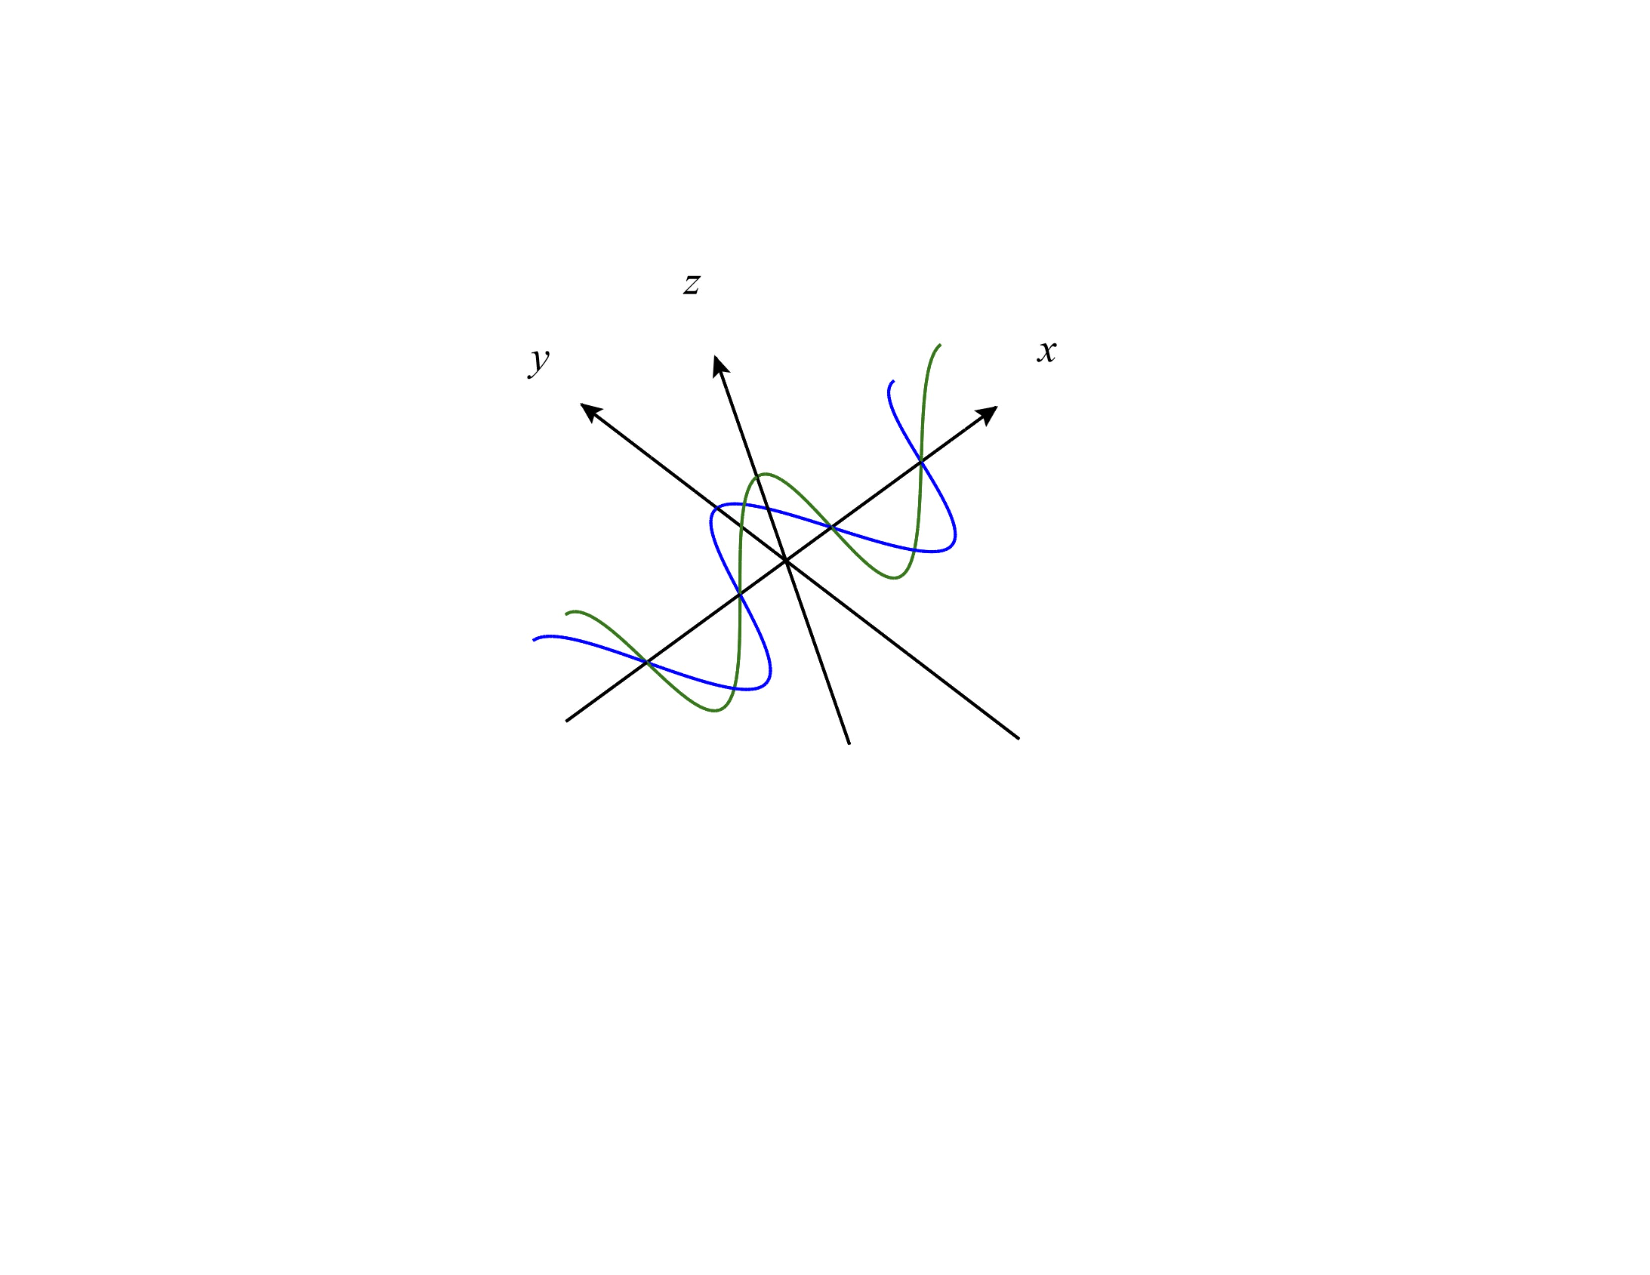
\includegraphics[width=.6 \textwidth]{./hw09_03_01.pdf}
\end{figure}

\item 
\[\hat{k} = \frac{1}{\sqrt{3}}(\hat{x} + \hat{y} + \hat{z}) \qquad \hat{n} = \frac{1}{\sqrt{2}}(\hat{x}-\hat{z})\]
\[\boxed{\vb{E} = \frac{1}{\sqrt{2}} E_0  e^{i((x+y+z)/\sqrt{3} -\omega t)} \, (\hat{x}-\hat{z})}\]
\[\vb{B} = \frac{1}{c}E_0 \Big(\frac{1}{\sqrt{3}}(\hat{x} + \hat{y} + \hat{z})\times \frac{1}{\sqrt{2}}(\hat{x}-\hat{z})\Big)e^{i((x+y+z)/\sqrt{3} -\omega t)}\]
\bigskip

Quick side note to do that cross-product:
\[(\hat{x} + \hat{y} + \hat{z}))\times (\hat{x}-\hat{z})\]
\[=[(\hat{x}\times\hat{x}) + (\hat{y}\times\hat{x}) + (\hat{z}\times\hat{x})] - [(\hat{x}\times\hat{z}) + (\hat{y}\times\hat{z}) + (\hat{z}\times\hat{z})]\]
\[=(-\hat{z} + \hat{y})-(\hat{y} + \hat{x})\]
\[=(-\hat{z}-\hat{x}) = -(\hat{z}+\hat{x})\]
\bigskip

Back to the derivation:
\[\boxed{\vb{B} = -\frac{1}{\sqrt{6} \, c	}E_0 e^{i((x+y+z)/\sqrt{3} -\omega t)}\, (\hat{x} + \hat{z})}\]
\begin{figure}[!ht]
    \centering
    \label{fig:03_01}
    \caption{EM wave for question 9.9 part b. This one is quick a bit more tricky to draw. the idea is that the Poynting vector is in the $(1,1,1)$ direction and the E and B parts oare in the proper planes orthogonal to each other. }
    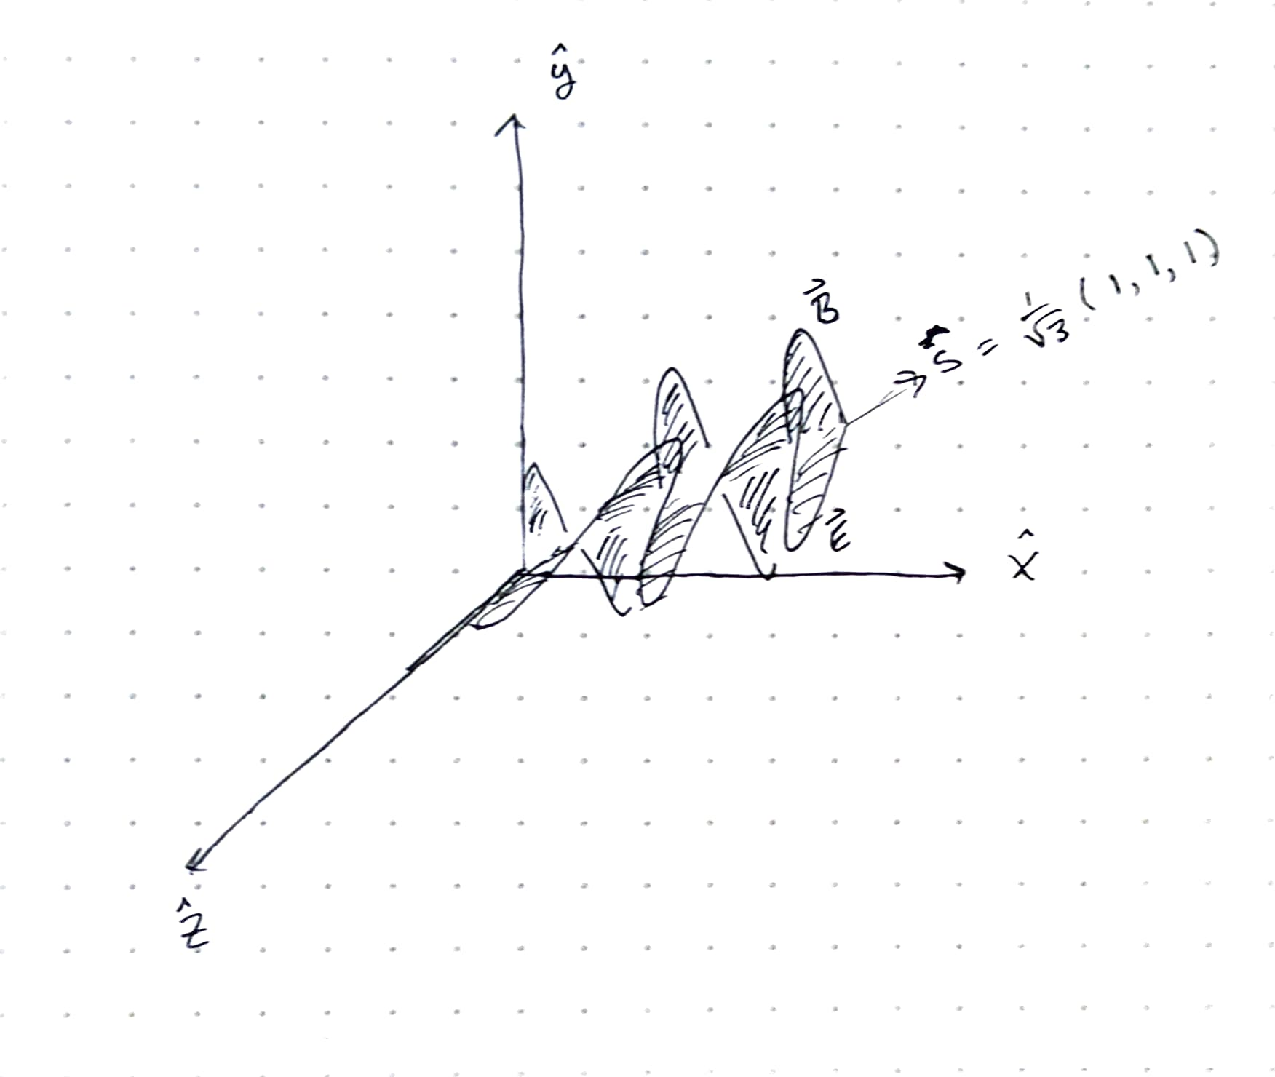
\includegraphics[width=.6\textwidth]{./hw09_03_02.pdf}
\end{figure}


\end{enumerate}



\end{document}